We model information preferences\textemdash preferences for taking or avoiding information\textemdash by applying and extending two theoretical approaches to modeling expectations-based reference-dependent preferences. One is the Disappointment Aversion (hereafter DA) approach pioneered by \citet{bellDisappointmentDecisionMaking1985}, with later contributions by \citet{loomesDisappointmentDynamicConsistency1986} and \citet{gulTheoryDisappointmentAversion1991}; the other is the Kőszegi and Rabin (hereafter KR) approach developed by Kőszegi and Rabin \citep{koszegiModelReferenceDependentPreferences2006,koszegiReferenceDependentRiskAttitudes2007}. In our exposition, we follow the notation of \citet{odonoghueChapterReferenceDependentPreferences2018} to discuss both approaches in a unified framework.

Formally, both approaches define the utility from a lottery of outcomes $L \equiv (x_1,p_1;x_2,p_2;...;x_N,p_N)$ given a reference lottery $R \equiv (r_1,q_1;r_2,q_2;...;r_M,q_M)$ as
\begin{equation*}
  U(L|R) \equiv \sum_{n=1}^{N} p_n[u(x_n)+v(x_n|R)],
\end{equation*}
where $u(x_n)$ is the intrinsic utility from lottery outcome $x_n$ and $v(x_n|R)$ is the gain-loss utility associated with that outcome. That is, $U(L|R)$ is the expected sum of intrinsic and gain-loss utility from each outcome of $L$.

The DA approach specifies the gain-loss utility from a specific outcome $x_n$ (from the lottery $L$) as
\begin{equation*}
  v(x_n|R) \equiv \mu (u(x_n)-\sum_{m=1}^M q_mu(r_m)),
\end{equation*}
i.e., as involving a comparison of the intrinsic utility of $x_n$ to the expected intrinsic utility from the reference lottery $R$. The gain-loss utility function $\mu(\cdot)$ is thereby specified as the piece-wise linear function
\begin{equation*}
  \mu(z)=
  \begin{cases}
    z          & \text{if } z \geq 0 \\
    \lambda z  & \text{if } z < 0 ,
  \end{cases}
\end{equation*}
where $\lambda>1$ (implying loss aversion). That is, if $u(x_n)$ is greater than $E[u(r_m)]$, this gives rise to gain utility $u(x_n)-E[u(r_m)]$, but if $u(x_n)$ is less than $E[u(r_m)]$, it gives rise to larger (in absolute terms) loss utility $\lambda(u(x_n)-E[u(r_m)])$.

In contrast, the KR approach specifies
\begin{equation*}
  v(x_n|R) \equiv \sum_{m=1}^M q_m \mu (u(x_n)-u(r_m));
\end{equation*}
that is, each outcome $x_n$ (from lottery $L$) is compared \emph{separately} to each individual outcome $r_m$ of the reference lottery $R$, giving rise (again with the same piece-wise linear gain-loss utility function) to gain utility $u(x_n)-u(r_m)$ if $u(x_n) \geq u(r_m)$ and to loss utility $\lambda [u(x_n)-u(r_m)]$ if $u(x_n)<u(r_m)$. The overall gain-loss utility $v(x_n|R)$ is the sum of all those separate gain and loss utility components, weighted by the probability $q_m$ of each outcome in $R$ that $x_n$ is compared to.

To make things more concrete and discuss the model in the context of preferences for information, consider our two cake eaters, Ana and Beto.\footnote{We emphasize that, in our example, Ana (who expects to receive information) and Beto (who expects not to receive information) are essentially the same person, except for their differing expectations.} Ana and Beto know that it is equally probable that the cake they are about to eat is either low- or high-calorie, and because they are both equally concerned about their calorie intake, their intrinsic utility of eating a high-calorie cake is \emph{low} ($\ell$), and their intrinsic utility of eating a low-calorie cake is \emph{high} ($h$). Furthermore, they do not anticipate being able to tell the cake’s calorie content from eating it, and, for now, they do not anticipate adjusting their behavior in response to the calorie information (i.e., the information is non-instrumental). Therefore, if they do not receive information about the calorie content of the cake, they will perceive eating the cake as yielding intrinsic utility $\half h + \half \ell$ (i.e., the probability weighted average of their utility in the low- and high-calorie states of the world).

Written in terms of lotteries, and for simplicity equating lottery outcomes with their induced utilities (i.e., skipping the intermediate step of mapping calories to intrinsic utilities), we can represent their situation if they currently do not know the cake's calorie content but will find out, as facing the lottery $L^i$ (superscript $i$ for \emph{informed}) equal to $(x_1=h,p=\half;x_2=\ell,p_2=\half)$. If they will \emph{not} find out, however, then they face the degenerate lottery $L^u$ (superscript $u$ for \emph{uninformed}) equal to $(x=\half h + \half \ell,p=1)$.

If their utility is reference-dependent, then their evaluation of these lotteries will depend on whether they \emph{expect} to be informed (i.e., see calorie information in the menu). For Ana, who expects to be informed, we can represent this as starting out with reference lottery $R^i=(r_1=h,q_1=\half;r_2=\ell,q_2=\half)$; for Beto, who expects not to be informed, we can represent this as starting with degenerate reference lottery $R^u=(r=\half h + \half \ell,q=1)$. Thus, there are four possible utilities:
\begin{itemize}
	\item $U(L^i|R^i)$ from expecting to be informed and getting information,
	\item $U(L^u|R^i)$ from expecting to be informed and not getting information,
	\item $U(L^i|R^u)$ from expecting to be uninformed and getting information, and
  \item $U(L^u|R^u)$ from expecting to be uninformed and not getting information.
\end{itemize}

An endowment effect is predicted if receiving the information is more valuable to a person who expects to receive it (like Ana) than to a person who does not expect to receive it (like Beto):\footnote{\citet{sprengerEndowmentEffectRisk2015} emphasizes that the KR endowment effect for risk that he tests for \enquote{should be thought of as distinct from the standard endowment effect literature documenting exchange anomalies as discrepancies between WTP and WTA for the same object. The KR endowment effect for risk is a risk preference discrepancy between risk taking when the referent is certain and risk taking when the referent is stochastic.} (p.1458) Similarly, in our context, the endowment effect for information is an information preference discrepancy between information seeking when the referent is certain (i.e., an agent does not expect to receive information, making the referent a degenerate lottery) and information seeking when the referent is stochastic (i.e., the agent expects to receive information, making the referent a non-degenerate lottery).}
\begin{equation}
  U(L^i|R^i)-U(L^u|R^i)>U(L^i|R^u)-U(L^u|R^u).
  \label{eq:endowmentEffect}
\end{equation}

Below we discuss four results regarding the existence of an endowment effect for information under the DA or the KR approach when information is either non-instrumental or instrumental. See Appendix \ref{appendix:theory} for all the derivations.

\begin{prop}
  Assume reference-dependent utility following the DA approach, with a piece-wise linear gain-loss utility function and non-instrumental information. For any lottery $L$, $U(L^i|R^i)-U(L^u|R^i)=U(L^i|R^u)-U(L^u|R^u)$. Therefore, no endowment effect is predicted.
  \label{prop:nonInstrumental-DA}
\end{prop}

\begin{figure}[ht]
  \caption{Value of information under the DA approach, with non-instrumental information.}\label{fig:nonInstrumental-DA}
  \begin{center}
  {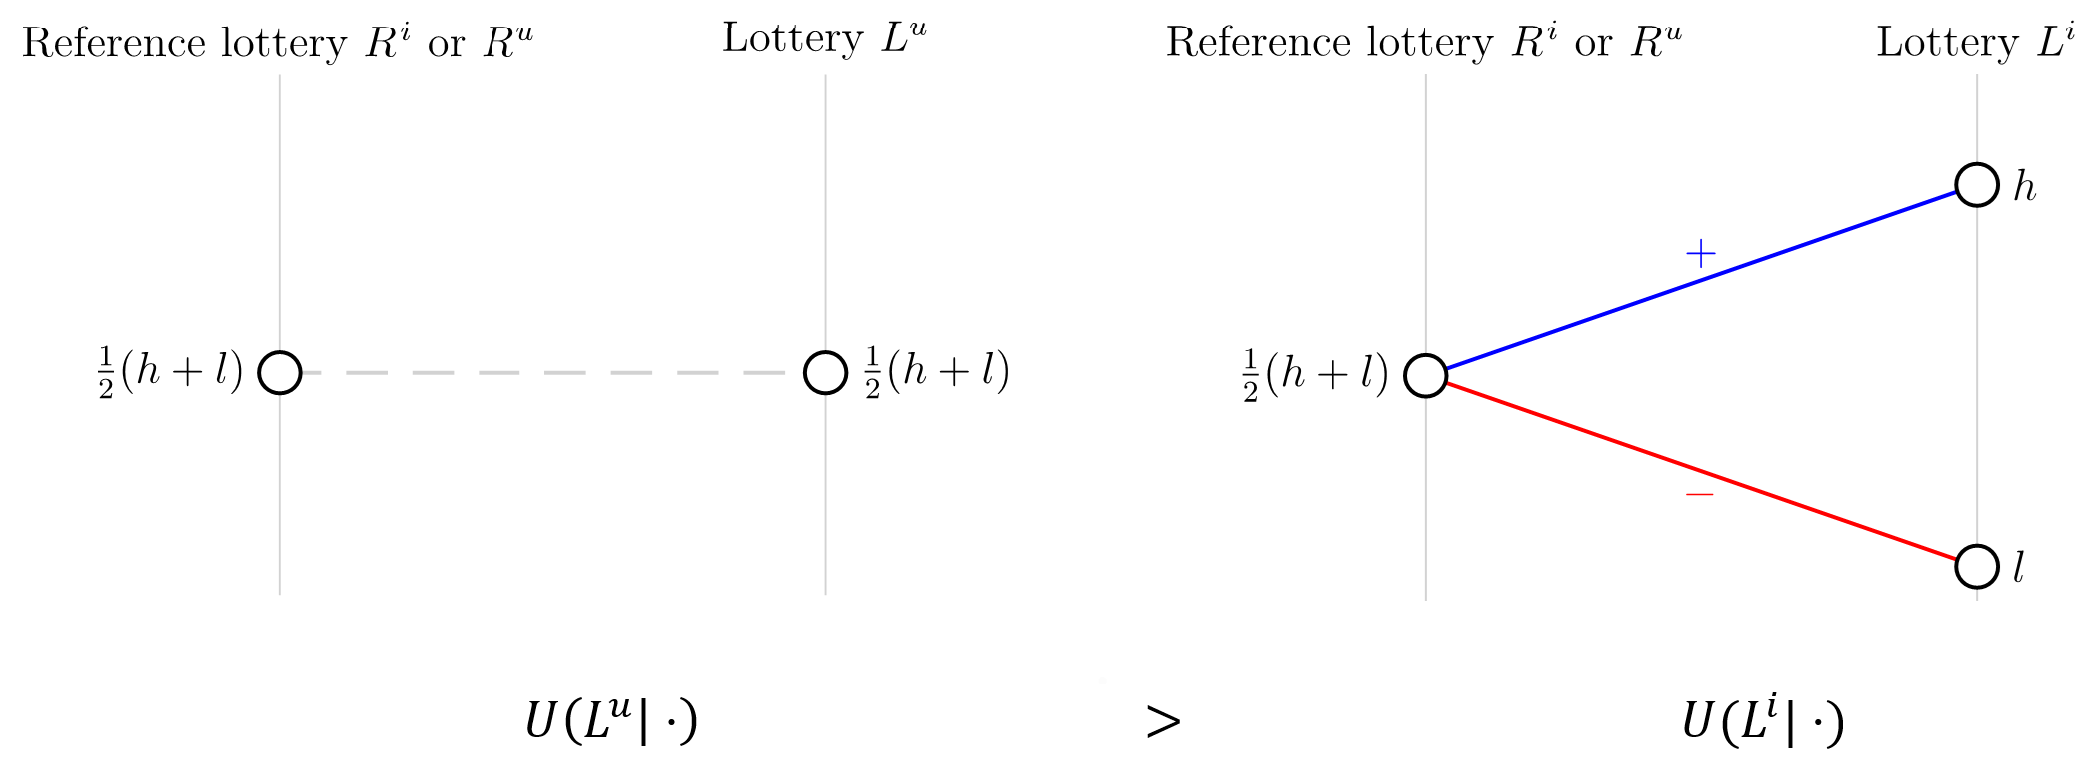
\includegraphics[width=1\textwidth]{./figures/theory_fig1.png}}
  \end{center}
\end{figure}

Because under the DA approach the reference lottery collapses to its expectation before evaluating gain-loss utility, and given that both referents $R^i$ and $R^u$ have the same expectation $E[R^i]=E[R^u]=\half(h+\ell)$, the difference $U(L^i|\cdot)-U(L^u|\cdot)$ is the same regardless of whether a person expects to receive information or not. Specifically, as illustrated in Figure \ref{fig:nonInstrumental-DA}, relative to not getting information (illustrated in the left panel), getting information (illustrated in the right panel) involves a gain of $h-\half(h+\ell)=\half(h-\ell)$ with probability one-half and a utility loss of $l-\half(h+\ell)=-\half(h-\ell)$ with probability one-half. Because of loss aversion, however, the utility loss receives additional weight $\lambda>1$, implying that $U(L^i|\cdot)-U(L^u|\cdot)=-\qrtr(\lambda-1)(h-\ell)<0$. In other words, the value of information is equally negative, regardless of expectations.

\FloatBarrier

\begin{prop}
  Assume reference-dependent utility following the KR approach, with a piece-wise linear gain-loss utility function and non-instrumental information. For any lottery $L$, $U(L^i|R^i)-U(L^u|R^i)>(L^i|R^u)-U(L^u|R^u)$. Therefore, an endowment effect is predicted.
  \label{prop:nonInstrumental-KR}
\end{prop}

\begin{figure}[ht]
  \caption{Value of information under the KR approach, with non-instrumental information.}\label{fig:nonInstrumental-KR}
  \begin{center}
  {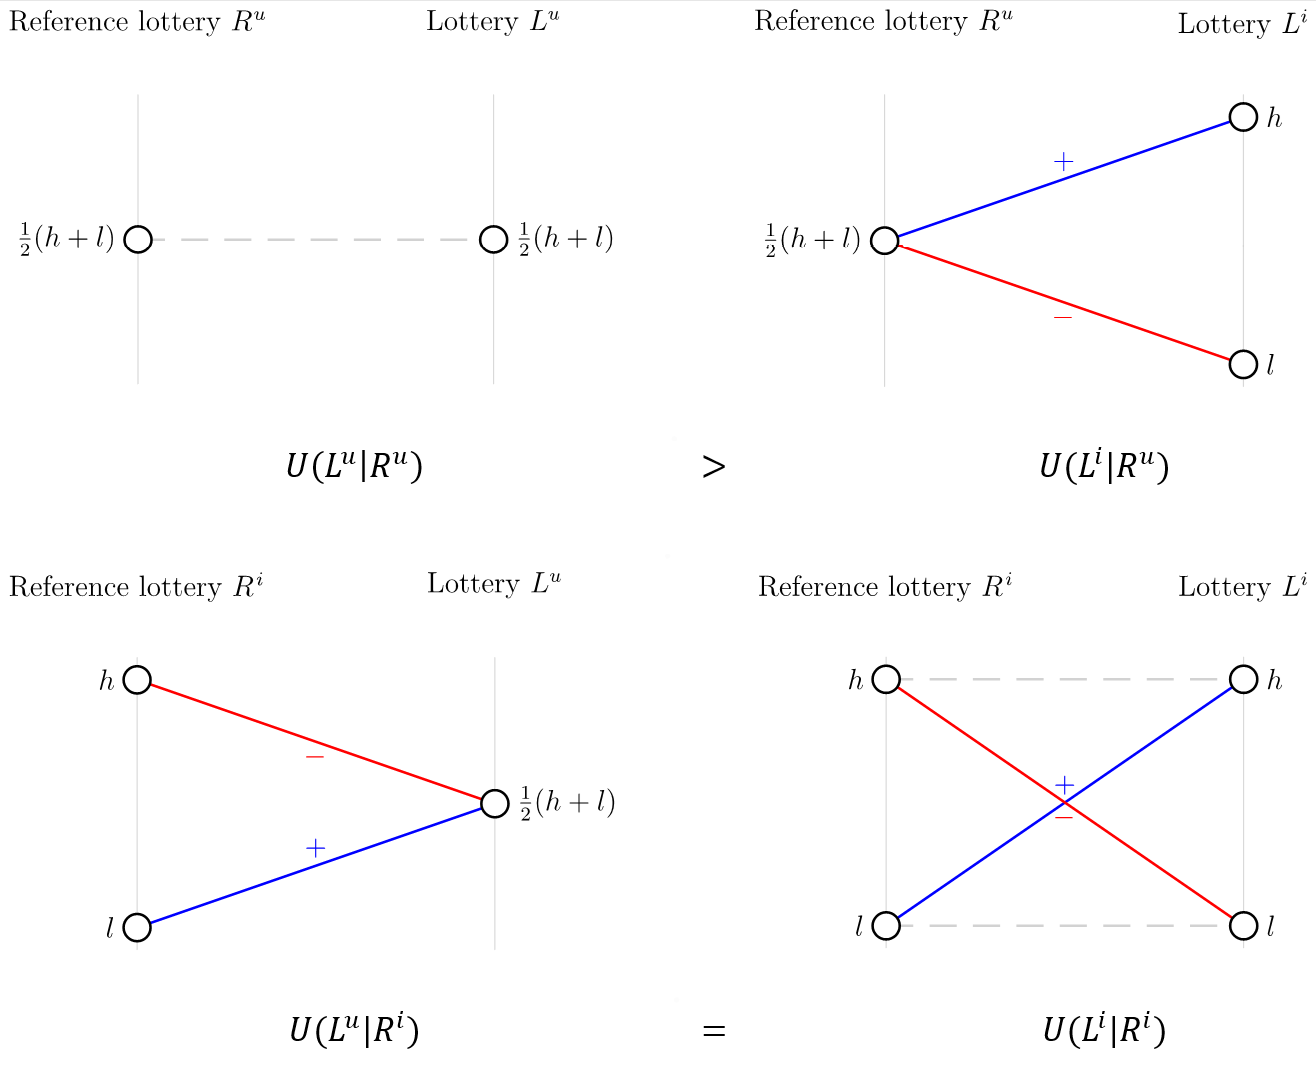
\includegraphics[width=1\textwidth]{./figures/theory_fig2.png}}
  \end{center}
\end{figure}

Figure \ref{fig:nonInstrumental-KR} illustrates how the endowment effect for information arises under the KR approach. Since all four possible outcomes yield the same intrinsic utility $\half(h+\ell)$, the endowment effect is driven by differences in gain-loss utility depending on expectations.

If information is not expected (illustrated in the top panels), getting it results in the same net utility loss $U(L^i|R^u)-U(L^u|R^u)=-\qrtr(\lambda-1)(h-\ell)<0$ as under the DA approach. In other words, Beto's value of information is negative\textemdash{he is information averse}.

If information is expected (illustrated in the bottom panels), then not getting it (the bottom-left panel) involves a utility gain of $\half(h+\ell)-\ell=\half(h-\ell)$ and a loss $\half(h+\ell)-h=-\half(h-\ell)$, each weighted by probability one-half. Because the loss receives additional weight $\lambda>1$, the net gain-loss utility is $-\qrtr(\lambda-1)(h-\ell)<0$. But\textemdash and this is key\textemdash getting information that is expected (the bottom-right panel) involves a \emph{twice larger} utility gain of $(h-\ell)$ and loss of $-(h-\ell)$, each weighted \emph{twice smaller} probability one-quarter, before applying outcomes $\ell$ in both. On net, then, the gain-loss utility ends up being the same $-\qrtr(\lambda-1)(h-\ell)<0$, implying that $U(L^i|R^i)-U(L^u|R^i)=0$. In other words, Ana's value of information is zero\textemdash{she is information neutral}.

Comparing Ana's and Beto's value of information, we find an endowment effect:
\begin{equation*}
  [U(L^i|R^i)-U(L^u|R^i)]-[U(L^i|R^u)-U(L^u|R^u)]=\qrtr(\lambda-1)(h-\ell)>0.
\end{equation*}
Note that, at least for non-instrumental information, the endowment effect does not make Ana value information more positively. Rather, it makes her value information \emph{less negatively}: she becomes information neutral rather than information averse.

Proposition \ref{prop:nonInstrumental-KR} is closely related to the prediction of an endowment effect for risk in \citet{koszegiReferenceDependentRiskAttitudes2007}. In fact, we have treated information in a way that parallels the way monetary risk is treated in their model: expecting to receive information is akin to having a stochastic referent, and expecting not to receive information is akin to having a non-stochastic referent.

The parallel extends further than Kőszegi and Rabin’s characterization of the psychology underlying their endowment effect for risk. They remark that their predictions crucially \enquote{do \emph{not} imply that a person is unbothered by risk she expects or faces, even if it does make her less risk averse.} Rather, a decisionmaker who had been expecting risk, or is already facing risk, \enquote{is already exposed to stochastic utility-decreasing sensations of loss, so taking additional risk does not add so much exposure to losses} (p. 1054). In our context, the endowment effect for information may arise similarly because those who expect information have already built utility-decreasing sensations of loss into their expected utility. In other words, those who expect information are more willing to get it, because they are already exposed to the potential pain of disappointment outweighing the potential joy of pleasant surprise.

\FloatBarrier

Up until this point, we have assumed that information is non-instrumental. Because of this, information has served a role only in determining whether a lottery is degenerate or not, making our application so far indistinguishable from applications analyzing monetary risk. However, information can serve the additional role of allowing people to adjust current and future choices in response to it. For example, if Ana or Beto learn the calorie content of the cake, they can decide to eat less or more of  it, or adjust how much they subsequently exercise.

Suppose for simplicity that these adjustments would increase their utility by the same amount $\Delta > 0$ in both states of the world, and define $h^* \equiv h+\Delta$ and $\ell^* \equiv \ell+\Delta$. Thus, given her expectation of learning the calorie content of the cake, Ana expects to be able to make adjustments and get intrinsic utility $\half(h^*+\ell^*)$. Assuming adjustments are not so large to turn bad news into good news, which requires $\Delta <\half(h-l)$, we then have propositions \ref{prop:instrumental-DA} and \ref{prop:instrumental-KR}.

\begin{prop}
  Assume reference-dependent utility following the DA approach, with a piece-wise linear gain-loss utility function and instrumental information. For any lottery $L$, $U(L^i|R^i)-U(L^u|R^i)>(L^i|R^u)-U(L^u|R^u)$. Therefore, an endowment effect is predicted.
  \label{prop:instrumental-DA}
\end{prop}

\begin{figure}[ht]
  \caption{Value of information under the DA approach, with instrumental information.}\label{fig:instrumental-DA}
  \begin{center}
  {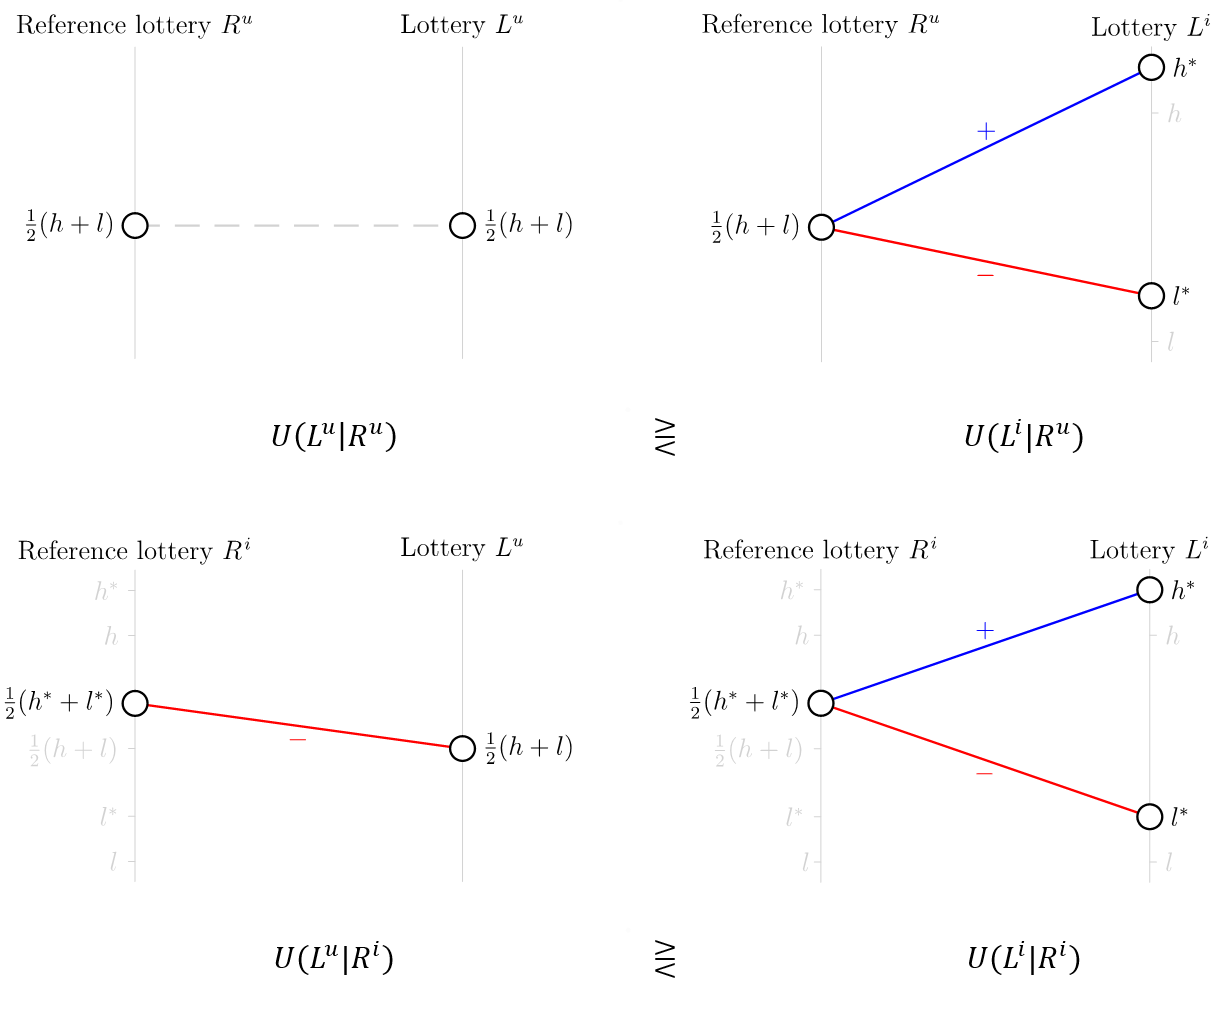
\includegraphics[width=1\textwidth]{./figures/theory_fig3.png}}
  \end{center}
\end{figure}

Figure \ref{fig:instrumental-DA} illustrates how the endowment effect now arises under the DA approach as well. The ability to make behavioral adjustments adds $\half \Delta + \half \Delta = \Delta$ to the intrinsic utility of getting information, regardless of expectations. If information is unexpected (illustrated in the top panels), however, then the gained ability to adjust enhances the gain from the good outcome and mitigates the loss from the bad outcome, thereby adding $\half \Delta + \half \lambda \Delta = \half (1 + \lambda) \Delta$ to gain-loss utility. The overall value of unexpected information becomes
\begin{equation*}
  U(L^i|R^u)-U(L^u|R^u)=-\qrtr(\lambda-1)(h-\ell)+\Delta +\half(1+\lambda)\Delta,
\end{equation*}
which for large enough $\Delta$ may be positive.

If information is expected (illustrated in the botoom panels), then the \emph{forgone} ability to adjust gives rise to loss utility $-\half \Delta - \half \lambda \Delta = -\lambda \Delta$ from \emph{not} getting information (the bottom-left panel). Because both the $R^i$ and $L^i$ lotteries shift up by the same amount $\Delta$, however, gain-loss utility from getting information (the bottom-right panel) is unchanged. The overall value of expected information therefore becomes
\begin{equation*}
  U(L^i|R^i)-U(L^u|R^i)=-\qrtr(\lambda-1)(h-l)+\lambda +\lambda \Delta
\end{equation*}

Moreover, because $\lambda>1$ implies that $\lambda \Delta > \half(1+\lambda)\Delta$, the value of expected information now exceeds that of unexpected information, implying an endowment effect. In short, the ability to adjust enhances the value of expected information by an avoided sure loss of $\lambda \Delta$, but the value of unexpected information by an avoided loss of $\lambda \Delta$ only with probability one-half, together with a gain of $\Delta$ with probability one-half. If losses outweigh gains, the former effect dominates.

\FloatBarrier

\begin{prop}
  Assume reference-dependent utility following the KR approach, with a piece-wise linear gain-loss utility function and instrumental information. For any lottery $L$, $U(L^i|R^i)-U(L^u|R^i)>(L^i|R^u)-U(L^u|R^u)$. Therefore, an endowment effect is predicted.
  \label{prop:instrumental-KR}
\end{prop}

\begin{figure}[ht]
  \caption{Value of information under the DA approach, with instrumental information.}\label{fig:instrumental-KR}
  \begin{center}
  {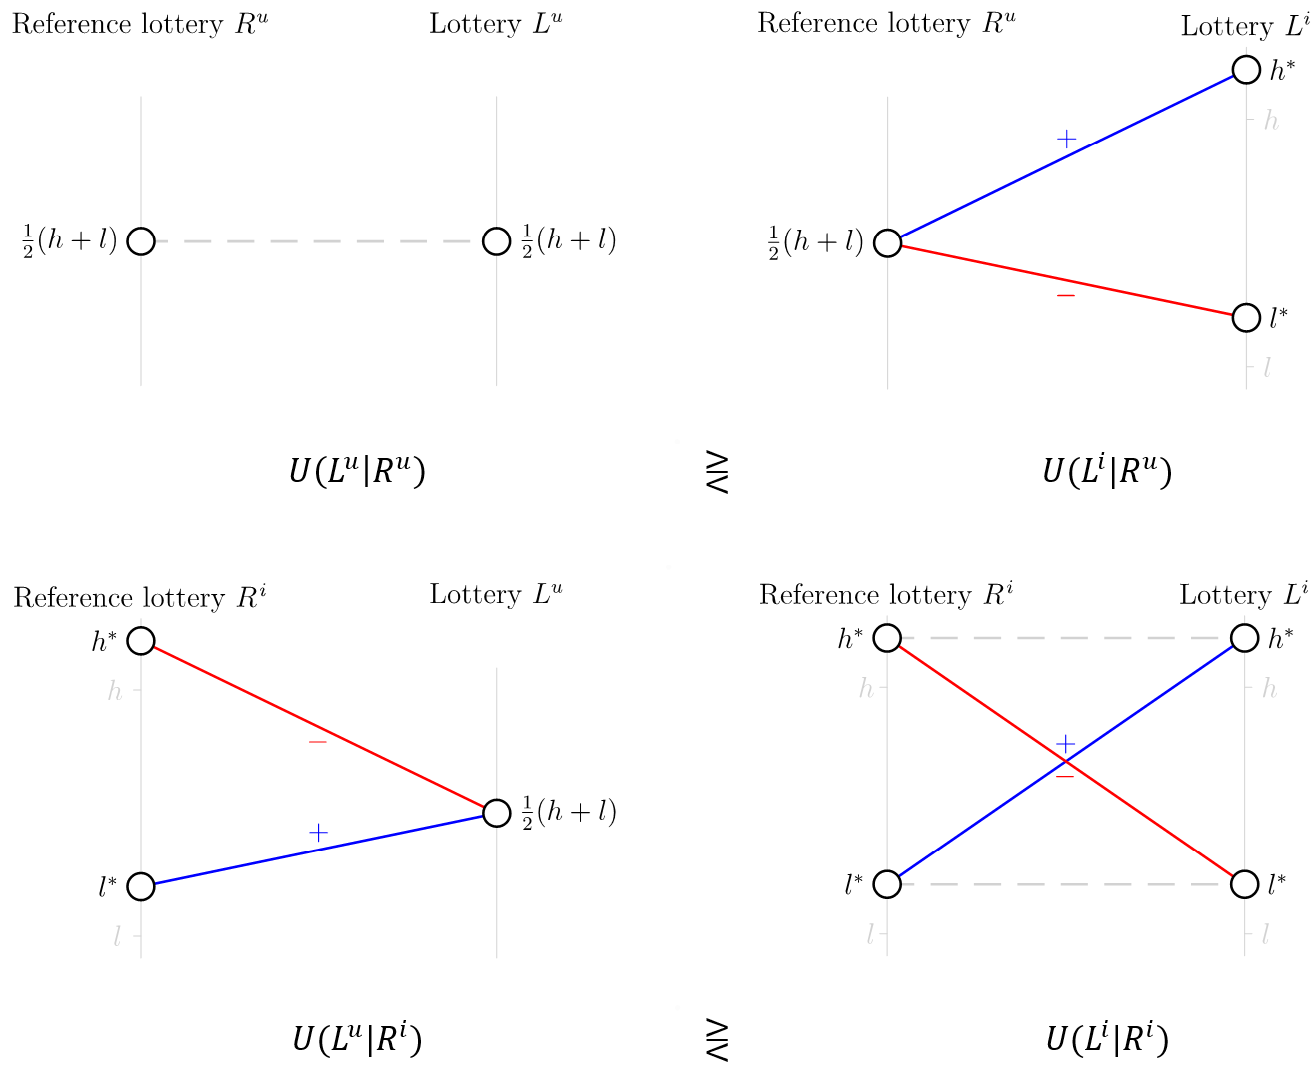
\includegraphics[width=1\textwidth]{./figures/theory_fig4.png}}
  \end{center}
\end{figure}

Figure \ref{fig:instrumental-KR} illustrates how the ability to adjust affects outcomes under the KR approach. As under the DA approach, it adds $\half \Delta + \half \Delta = \Delta$ to the intrinsic utility of getting information, regardless of expectations. Also as under the DA approach, it adds $\half (1+\lambda) \Delta$ to gain-loss utility from getting unexpected information (the top-right panel), making the overall value of such information
\begin{equation*}
  U(L^i|R^u)-U(L^u|R^u)=-\qrtr(\lambda-1)(h-\ell)+\Delta+\half (1+\lambda)\Delta.
\end{equation*}
Different from the DA approach, however, it enhances the value of \emph{not} getting expected information (the bottom-left panel) by an avoided loss of $\lambda \Delta$ only with probability one-half, together with a gain of $\Delta$ with probability one-half, resulting in the same addition of $\half(1+\lambda)\Delta$ to gain-loss utility overall. Moreover, because both the $R^i$ and $L^i$ lotteries shift up by the same amount $\Delta$, gain loss utility from getting information (the bottom-right panel) is again unchanged. The overall value of expected information therefore becomes
\begin{equation*}
  U(L^i|R^i)-U(L^u|R^i)=-\qrtr(\lambda-1)(h-\ell)+\Delta+\half (1+\lambda)\Delta,
\end{equation*}
which is identical to the value of unexpected information. The upshot is that the endowment effect $[U(L^i|R^i)-U(L^u|R^i)]-[U(L^i|R^u)-U(L^u|R^u)]$ stays the same: the implications of adjustments cancel out exactly.\footnote{Contrary to the result of Proposition \ref{prop:instrumental-DA}, this indifference result depends crucially on our simplifying assumption that adjustments to both the \enquote{good} and \enquote{bad} outcomes enhance utility by the same amount $\Delta$. More generally, if adjustments enhance the good outcome by $\Delta^h$ and the bad outcome by $\Delta^i \neq \Delta^h$, the endowment effect under the KR approach changes by $\qrtr(\lambda-1)(\Delta^h-\Delta^l) \neq 0$. Provided $\Delta^l<\qrtr(h-\ell)$, the overall endowment effect $\qrtr(\lambda-1)(h-\ell)+\qrtr(\lambda-1)(\Delta^h-\Delta^\ell)$ will remain positive.}

\FloatBarrier
